\chapter{Logging and the Write-Ahead Rule}
\label{ch:wal}

The buffer pool steals and does not force (\cref{ch:buffer}). So at the moment of
a crash, the disk can hold changes from transactions that never committed, and
can lack changes from transactions that did. The \term{log} is what lets the
engine repair both. This chapter explains what goes in it, and the one rule that
makes it trustworthy.

\section{The failure model}

\begin{description}[leftmargin=1.2em]
\item[Transaction failure.] A transaction aborts: a deadlock victim, a constraint violation, or the user's choice. Its effects must be removed.
\item[System failure.] The process or machine stops. Memory is lost; the disk survives. Committed work must reappear; uncommitted work must vanish.
\item[Media failure.] The disk is lost. Only a backup or a replica helps; it is outside the scope of the log alone.
\end{description}

The log handles the first two. It is an append-only file of \term{log records},
each describing one change, written sequentially, which is the access pattern
storage handles best.

\section{Undo and redo}

An update record carries enough to apply the change again (\term{redo}) and to
reverse it (\term{undo}). For a page-oriented engine that might be the bytes
before and after; for a triple store it can be logical: ``insert triple
(5, 7, 9)'', whose undo is ``delete (5, 7, 9)''.

Every record has a \term{log sequence number} (LSN), increasing, unique, and
often simply the record's byte offset in the log. Records of one transaction are
chained by a \term{prevLSN} field, so the engine can walk a transaction's history
backward when it must undo it.

Every page stores a \term{pageLSN}: the LSN of the last logged change applied to
it. The pageLSN is how recovery knows whether a logged change already reached
the page on disk: if pageLSN $\ge$ the record's LSN, it did.

\section{The write-ahead rule}

\begin{keyidea}
\textbf{Write-ahead logging (WAL).} (1) A page may be written to disk only after
every log record describing a change to it is durable: flush the log up to the
page's pageLSN first. (2) A transaction commits only when its commit record, and
therefore all its earlier records, are durable.
\end{keyidea}

Rule 1 makes steal safe: if an uncommitted change reaches the disk, its undo
information is already in the log. Rule 2 makes no-force safe: if a committed
change has not reached the disk, its redo information is already in the log.
Between them, every possible state of the disk after a crash can be repaired.

\begin{figure}[ht]
\centering
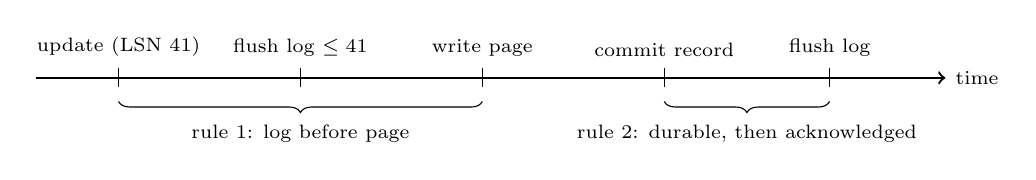
\begin{tikzpicture}[font=\scriptsize,x=1.05cm]
\draw[thick,->] (0,0) -- (11,0) node[right]{time};
\foreach \x/\l in {1/update (LSN 41),3.2/flush log $\le 41$,5.4/write page,7.6/commit record,9.6/flush log}{
  \draw (\x,0.12) -- (\x,-0.12); \node[above,align=center] at (\x,0.15) {\l};}
\draw[decorate,decoration={brace,amplitude=4pt,mirror}] (1,-0.3) -- (5.4,-0.3) node[midway,below=5pt]{rule 1: log before page};
\draw[decorate,decoration={brace,amplitude=4pt,mirror}] (7.6,-0.3) -- (9.6,-0.3) node[midway,below=5pt]{rule 2: durable, then acknowledged};
\end{tikzpicture}
\caption{The two orderings the write-ahead rule imposes.}
\label{fig:wal}
\end{figure}

\section{Making commits cheap: group commit}

Rule 2 means every commit waits for an \code{fsync} of the log. If each commit
issued its own \code{fsync}, throughput would be bounded by the device's
\code{fsync} rate. \term{Group commit} lets commits that arrive while a flush is
in progress share the next one:

\begin{lstlisting}[language=pseudo]
function Commit(txn):
  lsn = Append(commit record for txn)       // into the in-memory log buffer
  wait until persistentLSN >= lsn           // a background flusher wakes us

flusher loop:
  wait until someone asked, or a short interval passes
  batch = swap out the log buffer
  write(batch); fsync()                     // one fsync for many commits
  persistentLSN = last LSN in batch; wake all waiters
\end{lstlisting}

Under concurrency, the number of \code{fsync} calls grows much more slowly than
the number of commits. A single client still pays the full latency of one flush.

\section{When a record is damaged}

A crash can interrupt the last write to the log, leaving a \term{torn} record:
fewer bytes than its header promises. Bit rot or a misbehaving device can damage
a record whose bytes are all present. Robust logs detect both with two fields in
every record header: its \textbf{length}, so a short record is recognized, and a
\textbf{checksum} over its bytes, so a damaged one is. PostgreSQL, RocksDB, and
InnoDB all put a CRC on every log record. A recovery procedure then has a
policy choice, discussed in \cref{ch:durability}: stop at the first bad record
and keep everything before it, or refuse to start.

\begin{ontodb}[: log records and the log manager]
Every OntoDB log record has this layout (native byte order):

\begin{lstlisting}
u32 size       whole record, header included
u32 crc32c     over every byte after this field
u8  type       begin | commit | abort | update | clr | checkpoint | term | page
i64 lsn, i64 txn_id, i64 prev_lsn
then, by type:
  update       i32 page_id, u8 is_insert, u64 subject, u64 predicate, u64 object
  clr          the update fields, then i64 undo_next
  checkpoint   u32 n, then n active transaction ids
  term         u64 term_id, u32 n, then n bytes of canonical spelling
  page         i32 page_id, then the page's bytes after its pageLSN
\end{lstlisting}

The checksum is CRC-32C, the same checksum PostgreSQL, RocksDB, and InnoDB use.
A short buffer raises an ordinary storage error (a torn write), while a record
whose bytes are present but wrong raises a distinct corruption error, so the two
cases can be handled differently. LSNs start at 1; reopening a log continues
after its last valid record.

The log manager appends records to an in-memory buffer and a background thread
performs group commit; a test runs four threads committing twenty times each and
requires fewer \code{fsync}s than commits. A failed \code{fsync} is reported,
never retried, for the reason in \cref{ch:pages}.
\end{ontodb}

\begin{decision}{Length and CRC-32C in every record}
\dpart{Choice} Each record starts with its size and a CRC-32C over the rest. A
short record raises a storage error (a torn write); a full-length record with a
wrong checksum raises a distinct corruption error.
\dpart{Alternatives} No checksum; a plain CRC-32; a faster non-cryptographic
hash such as xxHash.
\dpart{Why} A crash leaves a torn tail, and the two cases deserve different
handling. CRC-32C has hardware instructions on x86 and ARM and is what
PostgreSQL, RocksDB, and InnoDB use.
\dpart{Cost} Eight bytes of header per record, and a checksum per append and per
read.
\end{decision}

\begin{decision}{LSNs are counters, not byte offsets}
\dpart{Choice} An LSN is a 64-bit counter starting at 1. On open, the next LSN
is one past the larger of the snapshot's LSN and the last valid record.
\dpart{Alternatives} Use the record's byte offset in the log, as ARIES and
PostgreSQL do, so an LSN locates its record directly.
\dpart{Why} A checkpoint of the memory database empties the log file. A counter
keeps increasing across that truncation, so ``skip records at or below the
snapshot's LSN'' stays correct; an offset would restart at zero.
\dpart{Cost} Finding a record by LSN needs a scan, not a seek.
\end{decision}

\begin{decision}{A failed \code{fsync} is fatal}
\dpart{Choice} When a log flush fails, the error is reported and the commit is
not acknowledged. The flush is never retried.
\dpart{Alternatives} Retry until it succeeds.
\dpart{Why} After a failed \code{fsync}, the kernel may have dropped the dirty
pages and cleared the error, so a retry that succeeds can still have lost the
data (\cref{ch:pages}).
\dpart{Cost} A transient device error stops the database instead of being
ridden out.
\end{decision}

\section{What a page record holds}

Rule 1 needs every change to a page to be logged before the page can be
written, and redo needs enough in each record to put the change back. There
are three common answers to ``what does the record hold''. \term{Physical}
logging records the bytes: a whole page image, or a byte range and its new
contents. \term{Logical} logging records the operation (``insert key $k$
into the SPO index''), and redo performs it again. \term{Physiological}
logging, which ARIES and most disk engines use, is a mix: the record names one
page (physical) and describes an operation on that page (logical), such as
``insert this key at slot 7 of page 12''.

Each choice moves work around. Page images are the simplest to redo (copy the
bytes) and need no knowledge of what is on the page, but they are large.
Logical records are small, but redo must run the operation against a structure
that may itself be damaged, which is why engines that log logically above the
page level still log pages physically below it.

\section{Changes that span pages}

A B+ tree split changes three pages: the old leaf loses its upper half, a new
leaf receives it, and the parent gains a separator. Each page gets its own
record. Suppose the log reaches the disk with the records for the two leaves
but not the parent's, and then the machine stops. Redo faithfully rebuilds
both leaves, and the parent still has no pointer to the new one. A full scan,
which walks the leaf chain, finds every key; a point lookup for a key in the
new leaf descends to the old leaf and misses. Nothing in the log is wrong, yet
the tree is.

The write-ahead rule is about single pages, so it cannot prevent this. A
multi-page change needs its own rule: its records must reach the log all
together or not at all. Systems get there in different ways:

\begin{description}[leftmargin=1.2em]
\item[Nested top actions (ARIES).] Log the split's page changes with undo information, then a dummy CLR that marks the split complete. If the crash comes before the dummy CLR, undo reverses the half-done split page by page.
\item[Mini-transactions (InnoDB).] Hold every latch the change took until it is finished, then append all its records to the log buffer in one step.
\item[Tolerate the half state (PostgreSQL).] B-link trees give every page a right link and a high key, so a search that lands on the old leaf can follow the right link. A split missing its parent pointer is legal, and the next writer that notices finishes it.
\end{description}

\begin{ontodb}[: page images and page groups]
OntoDB logs physically, by whole page. When a write guard on a page it changed
is released, still latched, the buffer pool appends a page record holding the
page's bytes after the pageLSN and sets the pageLSN to that record's LSN
(\code{BufferPoolManager::LogPageWrite}). Every page written through a guard
is covered by this one path: B+ tree nodes, tree headers, and the catalog.
Triple changes get a logical update record too, appended before the
statement changes any page; undo uses those (\cref{ch:aries}).

A tree \code{Insert} or \code{Remove} opens a \code{PageGroup} before its
first latch and closes it after its last. While a group is open, the log
manager writes nothing from the group's first LSN onward, so the flusher can
cut the log only between groups. The buffer pool, choosing a victim, passes
over any dirty page whose pageLSN is still held back, since writing it would
break rule 1. A test stops a tree at each named crash point inside a split or
a merge, flushes everything the log allows, copies the files, and checks that
redo yields a sound tree that holds either every key from before the
operation or every key from after it. Without page groups, all seven cases
fail.
\end{ontodb}

\begin{decision}{Whole page images, not physiological records}
\dpart{Choice} A page record carries the whole page after its pageLSN. Redo
copies it when the record is newer than the page.
\dpart{Alternatives} Physiological records, ``insert key $k$ at slot $i$ of
page $p$'', as ARIES and InnoDB use; byte-range diffs.
\dpart{Why} Redo needs to know nothing about the layout of a leaf, an internal
node, a header, or the catalog, so one short loop redoes them all, and a bug
in a page's code cannot also be a bug in its redo. The guard already knows
when a page changed; it does not know how.
\dpart{Cost} About 4 KB per page per operation. One triple touches at least
three trees, so it logs at least three pages, where its logical update
record is a few dozen bytes. A real engine would log diffs, or log a full
image only the first time a page changes after a checkpoint, as PostgreSQL's
full-page writes do.
\end{decision}

\begin{decision}{Page groups hold back the log, not the latches}
\dpart{Choice} A group marks its first LSN. The log does not flush past it, and
the pool does not evict a dirty page the group holds back, until the group
ends.
\dpart{Alternatives} Nested top actions with before-images and undo of an
unfinished split; InnoDB's mini-transaction, which keeps every page latched
until the end; B-link trees that accept a half split.
\dpart{Why} No before-images, no recovery pass for unfinished splits, and no
change to latching. Holding latches longer would have broken the tree's rule
that siblings are latched left to right, since a merge releases a page to
latch its left sibling.
\dpart{Cost} While any group is open, every later record waits too, so a
commit that arrives during a split waits for it. A group's pages cannot be
evicted, so the pool must hold more frames than the largest split touches. A
pool so small that every unpinned frame is held back cannot find a victim.
\end{decision}

\begin{status}
Log records (plan 8.1), the log manager with group commit (plan 8.2), and the
write-ahead rule with pageLSNs set on every change (plan 8.3) run. The rule
applies wherever a buffer pool is given a log manager: the recovery tests and
the crash harness. The shell's indexed backend is a temporary file and runs
without a log, and \code{ontodb <dir>} opens the memory database of
\cref{ch:durability}.
\end{status}

\begin{checkyourself}
\item State the two write-ahead rules, and say which buffer-pool policy each one makes safe.
\item A page has pageLSN 40. Recovery reads an update record for it with LSN 35. Redo it or skip it?
\item Ten sessions commit within one millisecond. Without group commit, how many \code{fsync}s? With it, at least how many?
\item A log's last record has a valid header claiming 60 bytes, and only 41 are in the file. Torn or corrupt? What if all 60 are there but the checksum fails?
\item Why does OntoDB number LSNs with a counter rather than a byte offset?
\item A split logs the old leaf, the new leaf, and the parent, in that order. Only the first two records reach the disk before a crash. After redo, which reads still work, and which fail?
\item Why may the buffer pool not evict a dirty page whose pageLSN is newer than the log's flushable LSN, even though it may wait for an ordinary log flush?
\item OntoDB logs whole page images. Name one thing this makes simpler and one thing it makes more expensive.
\end{checkyourself}

\section*{Further reading}
Mohan et al.\ \cite{aries}, sections 1--3; Gray and Reuter \cite{grayreuter},
chapters 9--10; Petrov \cite{petrov}, chapter 5.
